%this file is the second report
%a % comment anything after % until the end of the line

%minimum references to begin our article
\documentclass[12pt]{article}
\usepackage[english]{babel}
\usepackage[utf8]{inputenc}
\usepackage[T1]{fontenc}
\usepackage{graphicx}
\usepackage{fancyhdr}
\usepackage{hyperref}
\usepackage{float}
\usepackage{enumitem}
\usepackage{amsmath}
\usepackage[margin=1in]{geometry}
\usepackage{indentfirst}
\usepackage{titlesec}
\usepackage{verbatim}
\usepackage{url}
\usepackage{rotating}
\usepackage{caption}
\usepackage{pdfpages}

%for code
\usepackage{color}
\definecolor{grey}{rgb}{0.9,0.9,0.9}
\definecolor{teal}{rgb}{0.0,0.5,0.5}
\definecolor{violet}{rgb}{0.5,0,0.5}

\usepackage{listings}
\usepackage{listingsutf8}
\lstloadlanguages{[Visual]C++}
\lstdefinestyle{listing}{
  language=Java,
  captionpos=t,
  inputencoding=utf8/latin1,
  extendedchars=true,
  resetmargins=true,
%  xleftmargin=-60pt,
%  xrightmargin=-70pt,
%  frame=single,
  numbers=left,
  numberstyle=\tiny,
  numbersep=5pt,
  breaklines=true,
  breakatwhitespace=true,
  showspaces=false,
  showstringspaces=false,
  showtabs=false,
  tabsize=2,
  basicstyle=\footnotesize\ttfamily,
%  backgroundcolor=\color{grey},
  keywordstyle=\color{blue}\bfseries,
  commentstyle=\color{teal},
  identifierstyle=\color{black},
  stringstyle=\color{red},
  numberstyle=\color{violet},
}
\lstset{style=listing}


\newcommand{\sectionbreak}{\clearpage}

%\setlength{\parskip}{10pt plus 1pt minus 1pt} %Adds spacing between paragraphs 
\usepackage{parskip}
\setlength{\parindent}{15pt}

\usepackage{pifont}
\newcommand{\cmark}{\ding{51}}
\newcommand{\ajrn}{\ding{224}}
\newcommand{\xmark}{\ding{55}}

\pagestyle{fancy}
%\cfoot{Fast and furious game playing: Monte Carlo drift}
% the last extension makes it possible to add images

%presentation of the document
\title{Fast and Furious Game Playing: Monte Carlo Drift\smallbreak Final report} %not sure about the name of this report
\author{Prateek \textsc{Bhatnagar}, Gabriel \textsc{Prevosto}, \\
        Benoît \textsc{Viguier} \\
        \\
        Supervisors: Nikolaos \textsc{Parlavantzas}, Christian \textsc{Raymond}}
\date{02/02/2015}
\setlength\parindent{15pt}
\setlength\belowcaptionskip{-10pt}
\begin{document}
\maketitle

\begin{figure}[!h] 
\centerline{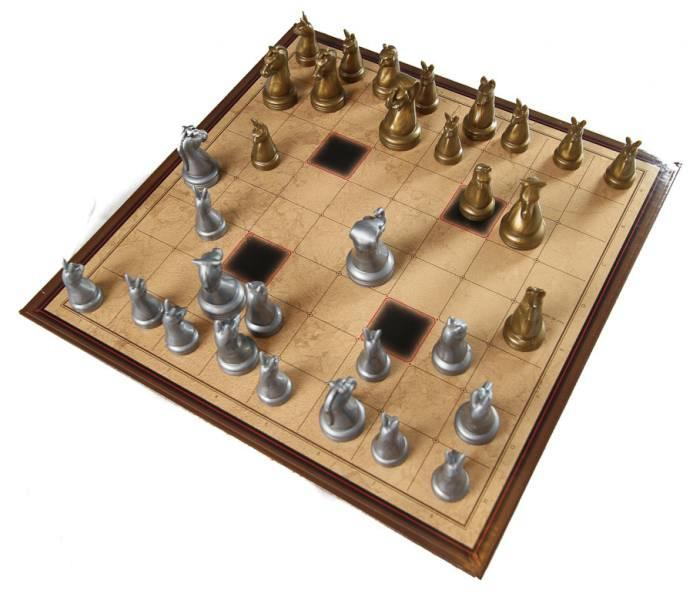
\includegraphics[scale=0.50]{Pictures/Arimaa}}
\end{figure}
\newpage

%to add a table of contents
\tableofcontents
\newpage


\section{Introduction}				\label{sec:introduction} 		The project is called \emph{Fast \& Furious Game Playing, Monte Carlo Drift}. Its purpose is to create an Artificial Intelligence able to compete against humans using the \emph{Monte Carlo Tree Search} algorithm.

We have chosen the game Arimaa because it is a two-players strategy board game not solved\footnote{A game solved is a game where good algorithms are able to find the perfect move in each situation to win, or to draw. For instance, \textit{Tic Tac Toe} or \textit{Draughts} are solved games.}.

A human plays a game by thinking of all possible moves as per one's imagination and then opts for the best amongst them. Before taking ones turn, a player can visualize ones options and predict how an opponent will counteract them. The algorithm will do the same by building a search tree containing the different posibilities. The Minimax algorithm does it by exploring all possibilities, which is heavy. The MCTS algorithm is lighter and converges to the Minimax algorithm, therefore it has been chosen for this project.

This algorithm will be parallelized in order to optimize it in a set of multi-core machines, allowing it to go further into the search tree, thus improving its efficiency.

Lorem ipsum dolor sit amet, consectetur adipisicing elit, sed do eiusmod
tempor incididunt ut labore et dolore magna aliqua. Ut enim ad minim veniam,
quis nostrud exercitation ullamco laboris nisi ut aliquip ex ea commodo
consequat. Duis aute irure dolor in reprehenderit in voluptate velit esse
cillum dolore eu fugiat nulla pariatur. Excepteur sint occaecat cupidatat non
proident, sunt in culpa qui officia deserunt mollit anim id est laborum.

\lhead{ }
\newpage
	\section{Achievements with respect to conceptualisation}			\label{sec:compare}			The project is called \emph{Fast \& Furious Game Playing, Monte Carlo Drift}. Its purpose is to create an Artificial Intelligence able to compete against humans using the \emph{Monte Carlo Tree Search} algorithm.

We have chosen the game Arimaa because it is a two-players strategy board game not solved\footnote{A game solved is a game where good algorithms are able to find the perfect move in each situation to win, or to draw. For instance, \textit{Tic Tac Toe} or \textit{Draughts} are solved games.}.

A human plays a game by thinking of all possible moves as per one's imagination and then opts for the best amongst them. Before taking ones turn, a player can visualize ones options and predict how an opponent will counteract them. The algorithm will do the same by building a search tree containing the different posibilities. The Minimax algorithm does it by exploring all possibilities, which is heavy. The MCTS algorithm is lighter and converges to the Minimax algorithm, therefore it has been chosen for this project.

This algorithm will be parallelized in order to optimize it in a set of multi-core machines, allowing it to go further into the search tree, thus improving its efficiency.

Lorem ipsum dolor sit amet, consectetur adipisicing elit, sed do eiusmod
tempor incididunt ut labore et dolore magna aliqua. Ut enim ad minim veniam,
quis nostrud exercitation ullamco laboris nisi ut aliquip ex ea commodo
consequat. Duis aute irure dolor in reprehenderit in voluptate velit esse
cillum dolore eu fugiat nulla pariatur. Excepteur sint occaecat cupidatat non
proident, sunt in culpa qui officia deserunt mollit anim id est laborum.

\newpage
  \section{Optimisations and results}        \label{sec:optimisations}    The project is called \emph{Fast \& Furious Game Playing, Monte Carlo Drift}. Its purpose is to create an Artificial Intelligence able to compete against humans using the \emph{Monte Carlo Tree Search} algorithm.

We have chosen the game Arimaa because it is a two-players strategy board game not solved\footnote{A game solved is a game where good algorithms are able to find the perfect move in each situation to win, or to draw. For instance, \textit{Tic Tac Toe} or \textit{Draughts} are solved games.}.

A human plays a game by thinking of all possible moves as per one's imagination and then opts for the best amongst them. Before taking ones turn, a player can visualize ones options and predict how an opponent will counteract them. The algorithm will do the same by building a search tree containing the different posibilities. The Minimax algorithm does it by exploring all possibilities, which is heavy. The MCTS algorithm is lighter and converges to the Minimax algorithm, therefore it has been chosen for this project.

This algorithm will be parallelized in order to optimize it in a set of multi-core machines, allowing it to go further into the search tree, thus improving its efficiency.

Lorem ipsum dolor sit amet, consectetur adipisicing elit, sed do eiusmod
tempor incididunt ut labore et dolore magna aliqua. Ut enim ad minim veniam,
quis nostrud exercitation ullamco laboris nisi ut aliquip ex ea commodo
consequat. Duis aute irure dolor in reprehenderit in voluptate velit esse
cillum dolore eu fugiat nulla pariatur. Excepteur sint occaecat cupidatat non
proident, sunt in culpa qui officia deserunt mollit anim id est laborum.
\newpage
  \section{Implementation of distribution}        \label{sec:distribution}    The project is called \emph{Fast \& Furious Game Playing, Monte Carlo Drift}. Its purpose is to create an Artificial Intelligence able to compete against humans using the \emph{Monte Carlo Tree Search} algorithm.

We have chosen the game Arimaa because it is a two-players strategy board game not solved\footnote{A game solved is a game where good algorithms are able to find the perfect move in each situation to win, or to draw. For instance, \textit{Tic Tac Toe} or \textit{Draughts} are solved games.}.

A human plays a game by thinking of all possible moves as per one's imagination and then opts for the best amongst them. Before taking ones turn, a player can visualize ones options and predict how an opponent will counteract them. The algorithm will do the same by building a search tree containing the different posibilities. The Minimax algorithm does it by exploring all possibilities, which is heavy. The MCTS algorithm is lighter and converges to the Minimax algorithm, therefore it has been chosen for this project.

This algorithm will be parallelized in order to optimize it in a set of multi-core machines, allowing it to go further into the search tree, thus improving its efficiency.

Lorem ipsum dolor sit amet, consectetur adipisicing elit, sed do eiusmod
tempor incididunt ut labore et dolore magna aliqua. Ut enim ad minim veniam,
quis nostrud exercitation ullamco laboris nisi ut aliquip ex ea commodo
consequat. Duis aute irure dolor in reprehenderit in voluptate velit esse
cillum dolore eu fugiat nulla pariatur. Excepteur sint occaecat cupidatat non
proident, sunt in culpa qui officia deserunt mollit anim id est laborum.
\newpage
  \section{Planning}        \label{sec:planning}    The project is called \emph{Fast \& Furious Game Playing, Monte Carlo Drift}. Its purpose is to create an Artificial Intelligence able to compete against humans using the \emph{Monte Carlo Tree Search} algorithm.

We have chosen the game Arimaa because it is a two-players strategy board game not solved\footnote{A game solved is a game where good algorithms are able to find the perfect move in each situation to win, or to draw. For instance, \textit{Tic Tac Toe} or \textit{Draughts} are solved games.}.

A human plays a game by thinking of all possible moves as per one's imagination and then opts for the best amongst them. Before taking ones turn, a player can visualize ones options and predict how an opponent will counteract them. The algorithm will do the same by building a search tree containing the different posibilities. The Minimax algorithm does it by exploring all possibilities, which is heavy. The MCTS algorithm is lighter and converges to the Minimax algorithm, therefore it has been chosen for this project.

This algorithm will be parallelized in order to optimize it in a set of multi-core machines, allowing it to go further into the search tree, thus improving its efficiency.

Lorem ipsum dolor sit amet, consectetur adipisicing elit, sed do eiusmod
tempor incididunt ut labore et dolore magna aliqua. Ut enim ad minim veniam,
quis nostrud exercitation ullamco laboris nisi ut aliquip ex ea commodo
consequat. Duis aute irure dolor in reprehenderit in voluptate velit esse
cillum dolore eu fugiat nulla pariatur. Excepteur sint occaecat cupidatat non
proident, sunt in culpa qui officia deserunt mollit anim id est laborum.
\newpage
	\section{Conclusion}			\label{sec:conclusion}			The project is called \emph{Fast \& Furious Game Playing, Monte Carlo Drift}. Its purpose is to create an Artificial Intelligence able to compete against humans using the \emph{Monte Carlo Tree Search} algorithm.

We have chosen the game Arimaa because it is a two-players strategy board game not solved\footnote{A game solved is a game where good algorithms are able to find the perfect move in each situation to win, or to draw. For instance, \textit{Tic Tac Toe} or \textit{Draughts} are solved games.}.

A human plays a game by thinking of all possible moves as per one's imagination and then opts for the best amongst them. Before taking ones turn, a player can visualize ones options and predict how an opponent will counteract them. The algorithm will do the same by building a search tree containing the different posibilities. The Minimax algorithm does it by exploring all possibilities, which is heavy. The MCTS algorithm is lighter and converges to the Minimax algorithm, therefore it has been chosen for this project.

This algorithm will be parallelized in order to optimize it in a set of multi-core machines, allowing it to go further into the search tree, thus improving its efficiency.

Lorem ipsum dolor sit amet, consectetur adipisicing elit, sed do eiusmod
tempor incididunt ut labore et dolore magna aliqua. Ut enim ad minim veniam,
quis nostrud exercitation ullamco laboris nisi ut aliquip ex ea commodo
consequat. Duis aute irure dolor in reprehenderit in voluptate velit esse
cillum dolore eu fugiat nulla pariatur. Excepteur sint occaecat cupidatat non
proident, sunt in culpa qui officia deserunt mollit anim id est laborum.
\newpage	

\end{document}
